% ============================================================
%  CRD 中文稿：对应英文 6 页版
%  编译：xelatex main_cn_6p.tex ×2
% ============================================================
\documentclass[10pt,twocolumn,a4paper]{ctexart}

\usepackage[margin=1.9cm]{geometry}
\usepackage{amsmath,amssymb}
\usepackage{graphicx}
\usepackage{booktabs}
\usepackage{caption}
\usepackage{needspace}
\usepackage[hidelinks]{hyperref}
\captionsetup{font=small,labelsep=quad}
\graphicspath{{../fig/}}

\setlength{\columnsep}{0.7cm}
\renewcommand{\figurename}{图}
\renewcommand{\tablename}{表}

\title{\bfseries CRD：面向全局图文错标检测的跨模态残差去偏}
\author{}
\date{}

\begin{document}
\maketitle

\begin{abstract}
\noindent
网页规模图文数据的清洗通常归结为对冻结视觉语言相似度取阈值，其前提是分数在不同图文对之间
可比。在受控基准的 Attribute 维度上，原始 CLIP 相似度把 $31.9\%$ 的 clean/noisy 组合排反，
尽管同一编码器区分两类样本的能力远高于随机。我们把这一现象部分归因于可从图像和文本特征
预测、且与是否匹配基本无关的加性分数成分。CRD（跨模态残差去偏）是一种事后校准：在冻结
特征上拟合两个小型加性头，并从标准化相似度中减去按比例缩放的估计成分；推理只需一对，不需要
参考库，标签只用于选择一个标量。我们还构建了 FGBench：由 COCO 与 Visual Genome 的五个事实
维度构成 $88{,}024$ 个 reciprocal cycle，标签为 silver。在三个报告的 Attribute 基座上，
CRD 提升 AUROC（CLIP ViT-B/16：$0.6806\to0.7187$；SigLIP2：$0.7026\to0.7509$）；$24$ 项
配对比较中 $21$ 项经 Holm 校正后显著，去除四个 GMM 单调重复后为 $17/20$ 个独立比较。两种
无参数去偏基线没有复现该增益。在 $32{,}000$ 行标注子集上，逻辑回归探针在 Attribute 和
Quantity 上分别高 $0.47$ 和 $1.60$ 点，MLP 在探索性 Action 维度上高 $7.62$ 点，代价约为
CRD 标签预算的四倍；在 CRD 的预算下，逻辑回归在 Attribute 上低 $4.36$ 点。方法按构造保持
cycle 级 2AFC 不变，并且在 Quantity 和 Entity 上没有超过 CSLS。
\end{abstract}

\noindent\textbf{关键词：}\emph{图文错标；跨模态相似度；分数校准；视觉语言模型；数据清洗；评测基准}

\section{引言}
\label{sec:intro-cn}

视觉语言模型已成为构建图文语料的标准工具：候选池被编码，每对得到一个相似度，低于阈值的
样本被丢弃或进入复标队列。这预设了相似度可以\emph{跨对}比较：得 $0.33$ 的对子比得 $0.25$
的对子更脏。该前提并不成立。图~\ref{fig:mot1} 给出一个反例：正确匹配对得 $0.252$，而把
动物数量写错的对子得 $0.331$，二者由同一冻结编码器打分。

现有检测器或改编码器，或改邻域。CSLS 用邻居集合重新规整分数，匹配头用学习到的分数替换
余弦；LEMoN 利用多模态邻居的一致性，TRACED 利用逐步编辑 caption 所形成的轨迹，判断图文对
是否为错配。它们改善的都是随后被取阈值的\emph{信号}，却留下同一个问题：信号固定时，两个互不相关的对子
是否共享同一尺度？在零样本 CLIP 家族内，容量并不能解决：ViT-L/14（$427.6$M 参数）在
Attribute 上的 AUROC 为 $0.6779$，而 ViT-B/16（$149.6$M）为 $0.6806$。缺的不是表示，
而是对“本不该进入全局比较的分数成分”的显式建模。

因此，我们把标准化相似度的可加性可预测部分写成
$g_\theta=a_\phi(u)+b_\psi(v)+b_0$，只使用每对自身的分数拟合，不使用标签；推理时减去
$z'=z-\lambda g_\theta$。编码器冻结，推理只消费一对，不需要参考库、配对 caption 或 cycle；
标签只用于选择 $\lambda$。我们在 FGBench 上评估，它包含来自 COCO 和 Visual Genome 的
$88{,}024$ 个 reciprocal cycle、五个事实维度。

\noindent\textbf{贡献。}
\begin{itemize}
  \item \textbf{方法}：CRD，一种事后校准，用两个轻量头估计图像侧和文本侧的加性分数成分，
  并从标准化相似度中减去；推理期不引入参考结构，改善全局判别。
  \item \textbf{基准}：FGBench，$88{,}024$ 个 reciprocal cycle、五个事实维度、明确划分卫生
  和自动化的划分/泄漏审计。
  \item \textbf{分析}：与五个同基座检测器和两种无参数去偏基线的配对检验、消融、选定的冻结
  基座，以及方法失效边界的明确说明。
\end{itemize}

\begin{figure*}[t]
  \centering
  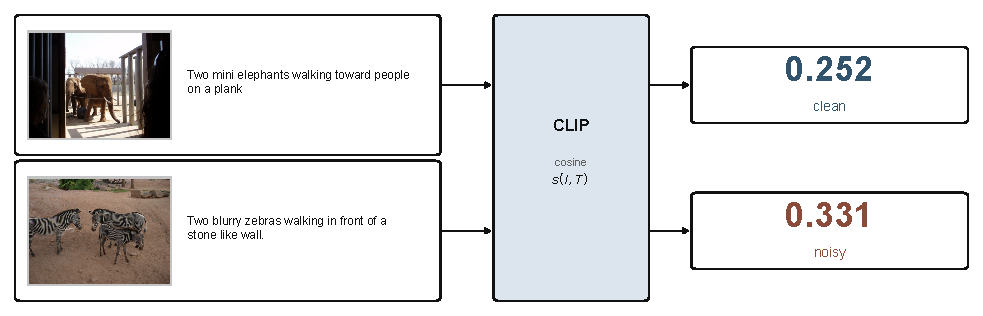
\includegraphics[width=\textwidth]{fig1_coco.pdf}
  \caption{原始图文相似度不能把正确对子排在错误对子之上。两对均来自 COCO Quantity 维度，
  由同一个冻结 CLIP ViT-B/16 打分，分数未作修改。上（正确匹配）为 $0.252$，下（数量写错）
  为 $0.331$。对原始分数取阈值会把两者判反。图像为 COCO 原图。}
  \label{fig:mot1}
\end{figure*}

\section{相关工作}
\label{sec:related-cn}

冻结对比编码器上的噪声检测沿三条路线展开。第一条重标定分数：CSLS~\cite{csls} 用邻居集合
校正 hubness，密度模型则拟合分数分布并对估计的噪声率取阈值。第二条用学习到的匹配器替换
分数，通常是在同一编码器上训练的图文匹配头。第三条利用关系结构：LEMoN~\cite{lemon} 用
多模态邻居判断一对是否匹配，TRACED~\cite{traced} 编辑 caption 并读取相似度轨迹。后两者
有效，但需要参考库、成批的其它对子或编辑模型；本文设定是一对进、一个分数出，没有其它样本。

检索中的分数不可比已有充分记录，常见补救是相对参考集重归一化、单调变换或拟合分布。与
CRD 的区别不在于加性——CSLS 也是加性的——而在于校正来源：CSLS 用参考库，我们的校正则
从每对自身的分数回归，可以在孤立一对上使用。单调变换不改变排序（GMM，表~\ref{tab:main-cn}）。
FOIL~\cite{foil} 与 SugarCrepe~\cite{sugarcrepe} 等组合性基准比较同一图像的两条 caption，
逐图偏移会抵消；这里比较的是两个互不相关的对子。

\section{问题与方法}
\label{sec:problem-cn}

\subsection{任务定义}
设 $f_I,f_T$ 为冻结图像/文本编码器，$u=f_I(I)$，$v=f_T(T)$，原始分数为余弦相似度
$s(I,T)=\operatorname{sim}(u,v)$；每对带二值标签 $y\in\{0,1\}$（clean/noisy）。任务是构造
$q(I,T)$，使其排序比 $s$ 更好。与同图候选排序不同，这里的比较是\emph{全局}的：两个对子
既不同图也不同文本；评分是\emph{对局部}的：$q$ 不能依赖当前还有哪些对子。因此分别报告
跨对 AUROC 与 cycle 内 2AFC。

\subsection{原始相似度的经验局限}
图~\ref{fig:mot1} 中，正确对子得 $0.252$，数量写错的对子得 $0.331$。单个例子不足以说明
问题；在 headroom 最大的 Visual Genome Attribute 上，把每个 clean 对与每个 noisy 对比较，
$31.9\%$ 的比较把 noisy 排在 clean 之上，即 $1-\mathrm{AUROC}$（$1-0.6806$）；Quantity 上
为 $16.9\%$（$1-0.8305$）。在一个 reciprocal cycle 内，固定图像替换 caption 会改变分数
（$0.324\to0.188$），固定 caption 替换图像也会改变（$0.324\to0.253$），说明分数取决于
具体图像和文本，而不只取决于是否对应。

\subsection{假设：加性分数成分}
设标准化分数分解为
\begin{equation}
  z=\underbrace{m(I,T)}_{\text{跨模态匹配}}+\underbrace{c(I,T)}_{\text{加性成分}},
  \label{eq:decomp-cn}
\end{equation}
其中 $c$ 可由 $u,v$ 预测，且与二者是否对应基本无关。更强的编码器提高第一项，但无关对子的
排序仍由第二项主导，这与 ViT-L/14 的 Attribute AUROC 不变一致。该分解也解释了为什么单调
重标定无效：它作用于整个 $z$。\eqref{eq:decomp-cn} 是建模假设，不是生成式解释；我们测试的
是其可操作推论：如果 $z$ 中有一部分可由 $u,v$ 预测，去掉这部分应改善全局判别，而拟合到
置换目标的对照不应改善。

\subsection{CRD 概览}
\label{sec:method-cn}
CRD 是事后校准层，不修改编码器，只增加两个小型头，并为单对返回校正分数。
图~\ref{fig:overview-cn}(a) 是训练路径：一对被编码为 $u,v$，两个特征送入加性头，头回归
该对的标准化相似度；图~\ref{fig:overview-cn}(b) 的推理复用同一编码器和头，通过一次减法
结合原始标准化分数与估计。编码器参数不更新，推理不观察标签。

\begin{figure*}[t]
  \centering
  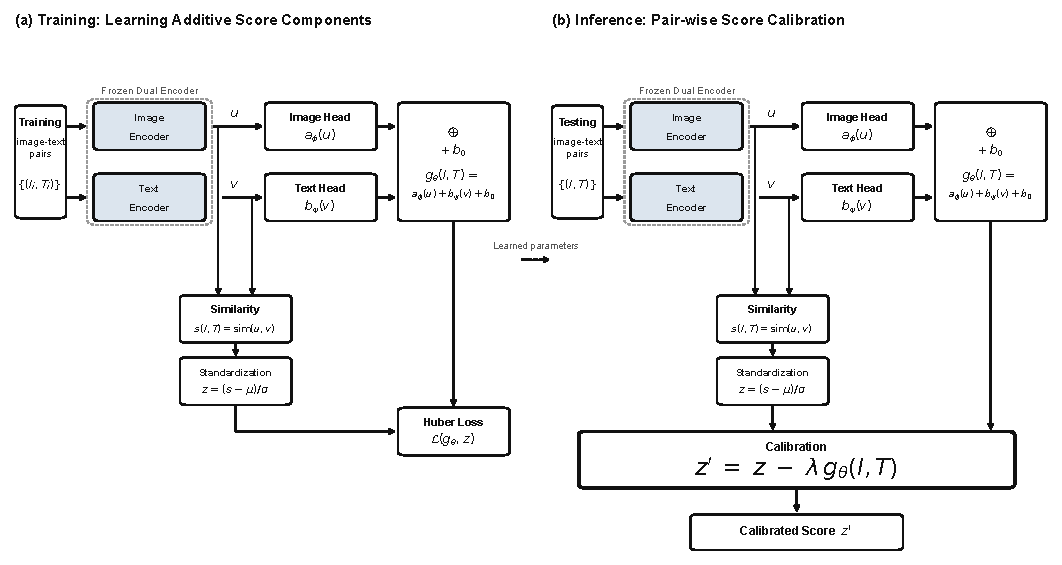
\includegraphics[width=\textwidth]{fig2_crd.pdf}
  \caption{CRD 总览。(a) 训练：从逐对标准化的图文相似度学习图像侧和文本侧加性成分；两个
  编码器冻结，只优化两个头和偏置 $b_0$。(b) 推理：从原始标准化相似度中减去估计成分；
  $\mu,\sigma$ 与头由训练固定，$\lambda$ 在验证集选取；只需一对，不需要参考库或 cycle。}
  \label{fig:overview-cn}
\end{figure*}

\subsection{冻结特征与分数标准化}
对一对 $(I,T)$ 计算
\begin{equation}
  u=f_I(I),\quad v=f_T(T),\quad s(I,T)=\operatorname{sim}(u,v),
\end{equation}
其中 $\operatorname{sim}$ 为余弦相似度。由于不同编码器的尺度不同，分数只用训练集统计量
标准化：
\begin{equation}
  \mu=\operatorname*{mean}_{\mathcal{D}_{\text{train}}}s,\quad
  \sigma=\operatorname*{std}_{\mathcal{D}_{\text{train}}}s+10^{-8},\quad
  z=\frac{s-\mu}{\sigma}.
  \label{eq:z-cn}
\end{equation}
验证和测试使用相同 $\mu,\sigma$，不在这些划分上重算。标准化使一个 $\lambda$ 网格可跨编码器
使用，并把目标放到残差尺度上。

\subsection{加性分数估计}
估计成分为两个头输出之和再加偏置：
\begin{equation}
  g_\theta(I,T)=a_\phi(u)+b_\psi(v)+b_0,
  \label{eq:g-cn}
\end{equation}
每个头是两层感知机，隐藏层宽度 $64$，激活为 GELU。保留加性形式而不是在拼接特征上拟合联合
残差网络，是因为联合网络可能吸收匹配项 $m(I,T)$；这是设计选择，不是数学必然。$g_\theta$
既不是第二个相似度，也不是图像或文本噪声的估计，而是只由两侧共同决定、没有跨侧交互项的
可预测成分。

\subsection{逐对目标与推理}
每个训练对只贡献一个目标：它自己的标准化分数 $z$：
\begin{equation}
  \mathcal{L}(\theta)=\frac{1}{|\mathcal{D}_{\text{train}}|}
  \sum_{(I,T)}\operatorname{Huber}\!\left(g_\theta(I,T),z(I,T)\right).
  \label{eq:loss-cn}
\end{equation}
用逐对分数而不是 cycle 均值监督是实质性的：同一 cycle 的匹配与不匹配样本共享 cycle 均值，
用均值作目标会让头去预测在被排序组内恒定的量。编码器冻结，只优化 $\phi,\psi,b_0$；回归
目标不含 clean/noisy 标签。标签只在选择 $\lambda$ 时进入，因此方法不是完全无监督，论文也不
这样描述。

校准分数为
\begin{equation}
  z'=z-\lambda g_\theta(I,T),
  \label{eq:calib-cn}
\end{equation}
其中 $\lambda\ge0$ 在验证集上通过最大化 $z'$ 的 AUROC 选择，网格为
$\Lambda=\{0,0.1,\dots,2.0\}$。网格包含零，验证可以选择不校准；在 placebo 运行中它确实
选择零。推理是对局部的：编码一次，计算两个头，返回 \eqref{eq:calib-cn}，不需要参考库、
配对 caption 或测试时阈值。两个头共 $65{,}795$ 个参数，耗时 $0.2$\,ms；端到端校准在
$15.1$\,ms 的 CLIP ViT-B/16 前向之外增加 $0.83$\,ms（$5.5\%$）。训练细节见
第~\ref{sec:exp-cn} 节。

\section{FGBench：基准构建}
\label{sec:fgbench-cn}

FGBench 问的是“两个互不相关的对子中哪一个更脏”，其构建直接来自这个问题。每张图和每条
caption 都是 COCO~\cite{coco} 或 Visual Genome~\cite{vg} 的已有条目；mismatch 通过违反
图像附带的结构化事实产生，因此标签有外部依据。划分在 cycle 级别不相交，构建过程可审计。

对图像对 $(A,B)$ 和 caption 对 $(T_A,T_B)$，生成四条记录：
\begin{equation}
\begin{aligned}
  &(A,T_A,\text{clean}),\quad (B,T_A,\text{noisy}),\\
  &(B,T_B,\text{clean}),\quad (A,T_B,\text{noisy}),
\end{aligned}
\end{equation}
称为一个 reciprocal cycle。每张图和每条 caption 各以一次匹配、一次不匹配出现，因此每个
维度严格 $50\%$ 平衡，两类在图像侧和文本侧分布相同；检测器不能利用图像或 caption 的频率
区分类别。cycle 是数据属性，不是方法属性：CRD 在单对上训练，在单对上推理。

五个维度来自两个数据源：COCO 构建 \textbf{Entity}（替换物体类别）与 \textbf{Quantity}
（替换数词）；Visual Genome 构建 \textbf{Attribute}（颜色、材料或状态）、\textbf{Action}
（谓词）和 \textbf{Relation}（空间或比较关系），均来自 VG150 风格标注。

\begin{table}[t]
\centering
\small
\setlength{\tabcolsep}{2pt}
\caption{FGBench v1-strict。每个 cycle 贡献两个匹配、两个不匹配对子，因此每个维度严格平衡。
所有方法使用同一 test split，共 $17{,}565$ 个 cycle、$70{,}260$ 个对子。}
\label{tab:fgbench-cn}
\begin{tabular}{llrrr}
\toprule
来源 & 维度 & Cycles & Pairs & Test (cycles) \\
\midrule
COCO          & Entity     & 32{,}589 & 130{,}356 &  2{,}298 \\
COCO          & Quantity   &  2{,}940 &  11{,}760 &    114 \\
Visual Genome & Attribute  & 49{,}042 & 196{,}168 & 14{,}281 \\
Visual Genome & Action     &    567   &   2{,}268 &    166 \\
Visual Genome & Relation   &  2{,}886 &  11{,}544 &    706 \\
\midrule
\multicolumn{2}{l}{合计}      & 88{,}024 & 352{,}096 & 17{,}565 \\
\bottomrule
\end{tabular}
\end{table}

标签是 silver：它们来自对结构化标注施加替换规则，而不是人工裁决。标注记录的是“标注了什么”，
不是图像的完整清单；未标注内容被视为未知而非不存在。strict 版本只保留 Relation 中有明确
标注支持的案例，并删除依赖六条歧义规则的 $276$ 个 cycle（$1{,}104$ 行）；本文所有数字均为
v1-strict。所有检测器在同一 manifest 上评估。基准审计报告：每张图和每条 caption 最多出现
在一个划分中，证据完整度 $1.000$。由于每张图和每条 caption 在两类中各出现一次，任何单侧
分数在两类上的条件分布相同；TF-IDF 检查因此是解析不变量（$0.5000$），不是独立经验证据，
而构造本身使纯文本捷径不可能成立。

\section{实验}
\label{sec:exp-cn}

\subsection{实验设置}
除非特别说明，所有方法共享同一个冻结 CLIP ViT-B/16 编码器；表~\ref{tab:main-cn} 各行只在
后处理和辅助输入上不同，表示相同；第~\ref{sec:cross-cn} 节在另外四个冻结编码器上重复比较。
头用 AdamW 优化 $1{,}500$ 次迭代，批大小 $256$，学习率 $10^{-3}$，权重衰减 $10^{-4}$，
Huber 损失使用默认转折点；三个种子共享固定训练子集、行序和由此得到的 $\mu,\sigma$，并核验
manifest、特征缓存和行序的哈希一致。主指标为跨对 AUROC，AUPRC 为辅；2AFC 单独报告，因为
它不能与 AUROC 互换。数值为三个种子的均值 $\pm$ 标准差（初始化变异；数据子集固定）。比较
使用以 cycle 为簇的配对 bootstrap，$5{,}000$ 次重采样，并在 $24$ 个单元上做 Holm 校正；
CSLS 的 $\lambda$ 在同一验证集上选择；在 $0$--$30$ 网格上重选不改变 Quantity/Entity 的
顺序。Action 的官方验证集只有两个 cycle，因此该维度只从训练 cycle 中划出 $20\%$（$399$ 中
的 $80$）作内部验证，且与保留 cycle 无共享图像；这是单次固定划分，属于协议偏差。其 $166$
个 test cycle 完全未动，Action 单元以 $\dagger$ 标注并作为探索性结果。

\subsection{与同基座检测器的比较}
表~\ref{tab:main-cn} 比较 CRD 与余弦阈值、CSLS、GMM 密度检测器、LEMoN（official）与
TRACED-style 复现、两种无参数特征去偏基线，以及作为参考上限的监督探针。两种去偏基线是
零假设：增益是否只来自去掉一阶特征结构。二者只在训练集拟合，不做梯度训练；唯一超参数
（ABTT 的 $k$）与 $\lambda$ 在同一验证集选择。LEMoN 使用官方适配器，并共享同一份缓存
CLIP 特征与 test split：IndexFlatIP、$k{=}5$、官方 $d_1+\beta d_n+\gamma d_m$ 分数，超参
在验证集拟合。TRACED 是机制级复现：构造三步、只删除内容的 caption 轨迹；由于没有复现
token 替换算子，它被视为下界。

\begin{table*}[t]
\centering
\footnotesize
\setlength{\tabcolsep}{7pt}
\caption{FGBench v1-strict test 上的 AUROC，所有行均为冻结 CLIP ViT-B/16。CRD 为三种子
均值 $\pm$ 标准差，基线为单次运行 AUROC。$^\dagger$Action 使用内部验证集。
GMM、均值中心化和 ABTT 是控制/去偏基线；LR 探针只在正文报告，不作为同预算检测器。
Holm 家族为五个方法行 $\times$ 五个维度减去 GMM/Action，共 $24$ 个单元；四个 GMM
单调重复单元扣除后为 $20$ 个独立比较。}
\label{tab:main-cn}
\begin{tabular}{lccccc}
\toprule
方法 & Entity & Quantity & Attribute & Action$^\dagger$ & Relation \\
\midrule
CLIP 余弦                & 0.9991 & 0.8305 & 0.6806 & 0.5913 & 0.5413 \\
CLIP + CSLS              & \textbf{0.9996} & 0.8882 & 0.6866 & 0.5869 & 0.5417 \\
LEMoN（official）          & 0.9990 & 0.8266 & 0.6755 & 0.5923 & 0.5218 \\
TRACED-style             & 0.9985 & 0.8412 & 0.6875 & 0.6102 & 0.5356 \\
\midrule
\multicolumn{6}{l}{\emph{对照（非检测器）}}\\
GMM（单调）              & 0.9991 & 0.8305 & 0.6806 & --- & 0.5413 \\
均值中心化余弦            & 0.9989 & 0.8570 & 0.6790 & 0.5890 & 0.5389 \\
ABTT 余弦                & 0.9985 & 0.8481 & 0.6765 & 0.5394 & 0.5464 \\
\midrule
\textbf{CRD（本文）}      & 0.9995$\pm$0.0000 & 0.8837$\pm$0.0011 & 0.7187$\pm$0.0001 & 0.6145$\pm$0.0009 & \textbf{0.5530}$\pm$0.0001 \\
\bottomrule
\end{tabular}
\end{table*}

Attribute 上，CRD 相对 seed-mean 余弦提升 $3.81$ 点（算术差；bootstrap 均值 $3.84$），
比表中五个方法/对照行高 $3.12$--$4.32$ 点，相对余弦的 95\% CI 为 $[3.73,3.96]$。
Quantity 的绝对增益更大（$+5.32$），但 CSLS 已解释其中大部分。Action 上 CRD 为 $0.6145$，
TRACED 为 $0.6102$，配对差 $+0.43$\,pp（95\% CI $[-1.75,2.54]$），未通过 Holm，因此主张
与 TRACED 相当而非更优。Quantity 和 Entity 上顺序在 seed-mean 口径下反转（CSLS $0.8882$
对 $0.8837$；$0.9996$ 对 $0.9995$；Entity 的 seed-mean 分数持平），因此不把 CRD 描述为
全面更优。$24$ 个单元中 $21$ 个经 Holm 显著；其中四个是 GMM 单调对照，其 AUROC 按构造与
余弦相同，因此独立计数为 $17/20$。例外为 Entity 对 CSLS、Quantity 对 CSLS、Action 对
TRACED。Entity 相对余弦虽然显著，但只有 $0.04$ 点，且所有方法都不低于 $0.9985$，
不视为实际增益。

与去偏基线的比较一致。作为独立的十项检验家族，CRD 在 seed-mean 分数上比均值中心化余弦高
$3.97$（Attribute）、$2.67$（Quantity）、$2.55$（Action）、$1.41$（Relation）、$0.06$
（Entity）点，比 ABTT 高 $4.22$、$3.56$、$7.51$、$0.66$、$0.10$ 点；Relation 对 ABTT 的
$+0.66$\,pp、CI $[-0.03,1.32]$ 是最弱的一格，不作为决定性证据。两种基线在 Attribute 上
都没有超过原始余弦（$0.6790$、$0.6765$ 对 $0.6806$），说明去掉一阶结构不能复现该增益。

\textbf{从排序到 top-$10\%$ 标签精度。} 这里的精度是被标记对子中 noisy 的比例。Attribute test 中最可疑的 $10\%$ 对子里，$84.9\%$ 为
noisy，余弦为 $76.8\%$，CSLS 为 $77.5\%$（相对余弦配对差 $+8.0$\,pp，算术差 $+8.1$；
cycle-clustered 95\% CI $[7.1,8.9]$）。其它维度不显著（$p=0.245$--$0.37$）；Entity 持平。
这是标签精度代理，不是下游训练收益的证据。

\textbf{监督参考。} 相同特征和训练子集也用于消费 pair 标签的探针：输入 $[u;v;u\odot v]$
的逻辑回归，以及 CRD 宽度的两层 MLP。它们不是同预算竞争者，但界定分类器能提取什么。
Attribute 上 LR 探针达到 $0.7234$，比 CRD 高 $0.47$\,pp（bootstrap CI $[0.28,0.60]$）；
MLP 为 $0.7214$。Quantity 上探针高 $1.60$，MLP 高 $1.85$；Action 上 MLP 高 $7.62$，
这里 $\lambda$ 在 $80$ 个内部验证 cycle 上选择。使用 $320$ 行预算时，Action LR 探针降到
$0.5687$（$-4.59$），MLP 仍为 $0.6517$（$+3.71$），因此预算惩罚依赖模型。Relation 上 MLP
过拟合并低于 CRD $3.93$。只用 $[u;v]$ 的探针处于随机水平（$0.5000$），这是 reciprocal
设计的必然结果：任何逐侧加性分数在一个 cycle 内给 clean 与 noisy 的和相同。$u\odot v$ 达到
$0.6977$：线性可提取信号在交互项中，逐侧非线性头只恢复一部分（$0.6944$/$0.6956$）。
用同样 $8{,}336$ 行预算训练时，LR 探针在 Attribute 降到 $0.6751$（相对 CRD $-4.36$），
Quantity 降到 $0.7949$（$-8.88$）：其先前优势使用 $32{,}000$ 行，约为 CRD 标签预算的四倍。

\textbf{头类型。} 同一加性形式的闭式 ridge 在 Attribute 和 Entity 上与 CRD 持平
（$0.7187$/$0.9996$），在 Quantity 高 $0.9$\,pp，在 Relation 持平，因此增益不需要非线性头。
拟合的 $g$ 在 Attribute 上达到 $R^2=0.326$，而 caption 长度和数字个数只达到 $R^2=0.005$，
说明它不是表面捷径。

\subsection{跨基座评估}
\label{sec:cross-cn}
\begin{table}[t]
\centering
\small
\setlength{\tabcolsep}{3.5pt}
\caption{CRD 在三个冻结基座上的 Attribute 结果（seed-mean AUROC；$\Delta$ 以点计）。
每个单元重新拟合头和 $\lambda$。}
\label{tab:cross-cn}
\begin{tabular}{llccc}
\toprule
基座 & 维度 & Raw & CRD & $\Delta$ \\
\midrule
CLIP B/16  & Attribute & 0.6806 & 0.7187 & +3.81 \\
CLIP L/14  & Attribute & 0.6779 & 0.7139 & +3.60 \\
SigLIP2    & Attribute & 0.7026 & 0.7509 & +4.83 \\
\bottomrule
\end{tabular}
\end{table}

表~\ref{tab:cross-cn} 报告三个 Attribute 基座。CRD 在这些单元上把原始 AUROC 提升
$+3.60$ 到 $+4.83$ 点；我们不对未展示的维度作外推。CLIP 内扩大规模几乎不改变 Attribute
（ViT-L/14，$2.9\times$ 参数，$0.6779$ 对 $0.6806$）。

\subsection{消融}
\begin{table}[t]
\centering
\small
\setlength{\tabcolsep}{5pt}
\caption{Visual Genome Attribute 上的消融（CLIP ViT-B/16，三种子均值）。所有行共享冻结
特征、训练划分和 $\lambda$ 网格。}
\label{tab:ablation-cn}
\begin{tabular}{lccc}
\toprule
配置 & AUROC & AUPRC & $\Delta$ (pp) \\
\midrule
CLIP 余弦（base）       & 0.6806 & 0.6680 & ---    \\
仅图像 $a_\phi(u)$      & 0.6944 & 0.6807 & +1.38  \\
仅文本 $b_\psi(v)$      & 0.6956 & 0.6904 & +1.50  \\
\textbf{加性（CRD）}     & \textbf{0.7187} & \textbf{0.7177} & \textbf{+3.81} \\
cycle 均值目标           & 0.7125 & 0.7077 & +3.19  \\
打乱目标（placebo）      & 0.6806 & 0.6680 & 0.00   \\
\bottomrule
\end{tabular}
\end{table}

表~\ref{tab:ablation-cn} 分离设计选择。仅图像 $0.6944$，仅文本 $0.6956$，加性为 $0.7187$；
两个单侧增益之和 $2.88$ 比联合增益 $3.81$ 小 $0.93$，说明两者互补而非重复。用 cycle 均值
监督损失 $0.62$ 点（$0.7125$），符合“目标在被排序组内恒定”的解释。placebo 用结构相同的头
拟合置换后的 cycle 均值，验证选择 $\lambda=0$，回到 $0.6806$。配对 bootstrap：加性减仅图像
$+2.43$\,pp，减仅文本 $+2.31$，减 cycle 均值 $+0.62$，减 placebo $+3.81$；所有种子符号一致，
最大离散 $0.15$\,pp。

\begin{table}[t]
\centering
\footnotesize
\setlength{\tabcolsep}{4pt}
\caption{同预算 joint-head 对照：相同缓存特征、1,500 步逐对目标、$\lambda$ 网格与三种子
（$65{,}795$ 对 $65{,}665$ 参数）。Action 因独立协议不纳入。加性列是同一缓存上的重跑，
相对表~\ref{tab:main-cn} 的差异最多为 $0.003$ AUROC（$0.3$ 点）。joint 把 Relation 2AFC 从
$0.6501$ 移到 $0.6535$；加性约束是足够的，而不是性能上限。}
\label{tab:joint-cn}
\begin{tabular}{lcccc}
\toprule
Head & Attribute & Quantity & Entity & Relation \\
\midrule
加性（CRD） & 0.7187 & 0.8866 & 0.9995 & 0.5538 \\
Joint $[u;v]$ & 0.7182 & 0.8759 & 0.9991 & 0.5537 \\
$\Delta$ & $-0.05$ & $-1.07$ & $-0.04$ & $-0.01$ \\
\bottomrule
\end{tabular}
\end{table}

\subsection{校准改变了什么、没有改变什么}
这里的 2AFC 是 cycle 级组比较：对每个 cycle，比较两个 clean 分数之和与两个 noisy 分数之和。
一个 cycle 内两侧涉及相同两张图和两条 caption，因此对 \eqref{eq:calib-cn} 求和得到
\begin{equation}
  \Delta'=\Delta-\lambda\Big[\sum_{\text{clean}}(a+b+b_0)
  -\sum_{\text{noisy}}(a+b+b_0)\Big],
\end{equation}
括号内恒为零，因为两个和都包含 $a(u_A)+a(u_B)+b(v_A)+b(v_B)+2b_0$。任何加性校正都保持该
指标不变，对任意 $a,b,\lambda$ 成立。CRD 的 2AFC 按构造等于余弦（Attribute $0.8282$，
$11{,}827/14{,}281$ cycles；Quantity $0.9649$；Entity $1.0000$ 饱和；Action $0.7831$，
$130/166$；Relation $0.6501$）；CSLS 同理不变。

不变性是指标属性，不说明校准无害，也不扩展到同图候选比较：那里只有固定侧的头会抵消。
去偏基线从另一方向说明问题：均值中心化和 ABTT 余弦不是可分离的加性校正，会改变该指标，
Attribute 上最多 $0.0089$，Action 上最多 $0.1686$。单调重标定不能被 AUROC 与余弦区分
（GMM 行），但其 2AFC 在 Attribute 和 Quantity 上分别移动 $-1.24$ 和 $-3.51$ 点。因此
两个指标都报告。

\subsection{外部迁移}
在 COCO Entity 上拟合的头在五个协议上应用，不使用目标标签或统计量。CRD 在 SugarCrepe 上
比余弦高 $+5.08$，Flickr noun $+1.04$，FOIL $+0.95$，Flickr random $+0.18$，在 MM-IMDb
上低 $0.35$；只用 VG Attribute 源时，只有 SugarCrepe 显著为正（$+0.98$）。目标混合了两个
同图准确率和三个行级 AUROC，因此迁移依赖源。监督探针从未显著更好，纯 caption 分类器处于
随机水平（$0.45$--$0.54$）；SugarCrepe 增益由文本侧头承载，作为边界报告。

\subsection{局限}
\eqref{eq:decomp-cn} 断言存在可预测的加性成分，并不声称该成分可识别为图像或文本偏差。
标签是 silver：替换规则有已知失败模式，且没有大规模人工裁决。Relation 的绝对值仍低：
最好 AUROC 为 $0.5530$，提升 $1.17$ 点。Quantity 和 Entity 上 CSLS 仍领先；Action 上 CRD
与 TRACED 统计不可区分。监督分类器在三个维度上更强，但需要全量训练集而非验证集；CRD 是
轻标签预算下的校准，不是最先进的监督检测。

\section{结论}
\label{sec:conclusion-cn}

全局 clean/noisy 检测预设两个互不相关的对子共享相似度尺度。本文记录了该预设在一个冻结
编码器下失效的实例（Attribute 上 $31.9\%$ 的比较排反），并把部分效应归因于可由图像和文本
特征预测的分数成分。CRD 用两个加性头估计该成分，不更新编码器、不使用参考库、除 $\lambda$
外不消费 pair 标签。

在 FGBench 上，该校准在三个报告的 Attribute 基座上改善 AUROC，并使 cycle 级 2AFC 不变。
FGBench manifest、审计工件与 CRD 实现将在接收后公开。消融把增益定位在两侧联合和逐对回归
目标上；打乱对照完全消除增益；两种无参数去偏基线没有复现 Attribute 增益。边界同样明确：CSLS 在 Quantity 和 Entity 上仍领先；Action 对 TRACED 不显著；
关系冲突仍困难；标签仍是 silver。

% ============================================================
\begin{thebibliography}{99}
\small
\bibitem{clip} Radford A, Kim J W, Hallacy C, et al. Learning transferable visual models from natural language supervision. ICML, 2021.
\bibitem{blip} Li J, Li D, Xiong C, et al. BLIP: Bootstrapping language-image pre-training for unified vision-language understanding and generation. ICML, 2022.
\bibitem{siglip} Zhai X, Mustafa B, Kolesnikov A, et al. Sigmoid loss for language image pre-training. ICCV, 2023.
\bibitem{coco} Lin T Y, Maire M, Belongie S, et al. Microsoft COCO: Common objects in context. ECCV, 2014.
\bibitem{vg} Krishna R, Zhu Y, Groth O, et al. Visual Genome: Connecting language and vision using crowdsourced dense image annotations. IJCV, 2017.
\bibitem{csls} Conneau A, Lample G, Ranzato M A, et al. Word translation without parallel data. ICLR, 2018.
\bibitem{foil} Shekhar R, Pezzelle S, Klimovich Y, et al. FOIL: A dataset for learning to compose phrase grounding and referring expressions. ACL, 2017.
\bibitem{sugarcrepe} Hsieh C Y, Zhang J, Ma Z, et al. SugarCrepe: Fixing hackable benchmarks for vision-language compositionality. NeurIPS Datasets and Benchmarks, 2023.
\bibitem{lemon} Zhang H, Balagopalan A, Oufattole N, et al. LEMoN: Label error detection using multimodal neighbors. arXiv:2407.18941, 2024.
\bibitem{traced} Afriat G, Lucas R, Meng X, et al. Seeing what's wrong: A trajectory-guided approach to caption error detection. ICLR, 2026.
\end{thebibliography}

\end{document}
